\documentclass{article} % For LaTeX2e
\usepackage{mltemplate,times}
\usepackage{hyperref}
\usepackage{url}
\usepackage{cite}
\usepackage{graphicx}
%\documentstyle[nips13submit_09,times,art10]{article} % For LaTeX 2.09


\title{Proposal: A simple PCANet-CNN for Image classification}

\setlength\belowcaptionskip{2pt}

\author{
Yin Zhang \\
Department of Statistics\\
University of Virginia\\
Charlottesville, VA 22903 \\
\texttt{yz4an@virginia.edu} \\
\And
Haoran Liu \\
Department of Computer Science \\
University of Virginia\\
Charlottesville, VA 22903  \\
\texttt{hl4fb@virginia.edu} \\
}

% The \author macro works with any number of authors. There are two commands
% used to separate the names and addresses of multiple authors: \And and \AND.
%
% Using \And between authors leaves it to \LaTeX{} to determine where to break
% the lines. Using \AND forces a linebreak at that point. So, if \LaTeX{}
% puts 3 of 4 authors names on the first line, and the last on the second
% line, try using \AND instead of \And before the third author name.

\newcommand{\fix}{\marginpar{FIX}}
\newcommand{\new}{\marginpar{NEW}}

\nipsfinalcopy % Uncomment for camera-ready version

\begin{document}

\maketitle

\begin{abstract}
%Our proposal is mainly motivated by the PCANet proposed in\cite{chan2015pcanet}, where the PCA filters are learned by extracting the principal components of the image patches. The features learned by PCA filters are on par with, sometimes even better than the most state of the art algorithms. In our proposal, 

In this paper, we are going to propose a simple deep learning architecture for image classification which is based on the PCANet \cite{chan2015pcanet}. In the proposed architecture, we extend the PCANet by connecting it with a convolutional network \cite{krizhevsky2012imagenet}, and the convolutional filters can be learned from back propagation. We will test the proposed deep network in various tasks such as objection recognition, digit recognition and face verification.
\end{abstract}

\section{Motivation and Overview}
This work is mainly motivated by the PCANet, which served as a simple but competitive deep learning baseline. Typically the deep learning networks (DNN) contains stacked trainable stages and is then followed by a supervised loss function. Each stage comprises a fully-connected layer or convolutional layer together followed by a nonlinear neuron function. DNN usually needs time-consuming training via back propagation.

In contrast, PCANet comprises only very basic data processing components. The multi-stage filters are learned by a simple principal component analysis, and no linear operation is involved until its very last layer, where binary hashing and histogram are employed to compute the features. Thus, back propagation is not needed for parameters updating and this results in a very efficient model training. The architecture of PCANet is shown in Figure 1.

Our goal is to design a novel deep learning architecture, which starts with a PCANet, without binary hashing and histogram, and then followed by a convolutional network and a supervised loss such as SVM loss or cross entropy loss. Our idea is as follows: the first two stages of PCANet already have learned a very good representation of each image, however, the binary hashing and histogram may lose some information. Therefore, we followed it with convolutional layer(s) and hope it can retain as much information as possible, thereby lead to a better performance. Since the input features of the convolutional layer(s) are well learned (by PCANet), so we guess it will not take too much time to train the these convolutional filters. However, we haven't decided the architecture of convolutional layers yet, but the number of convolutional layers would not exceed 2.



%\section{Previous work}
%PCANet, CNN

\begin{figure}[h]
\vspace{-15pt} \centering
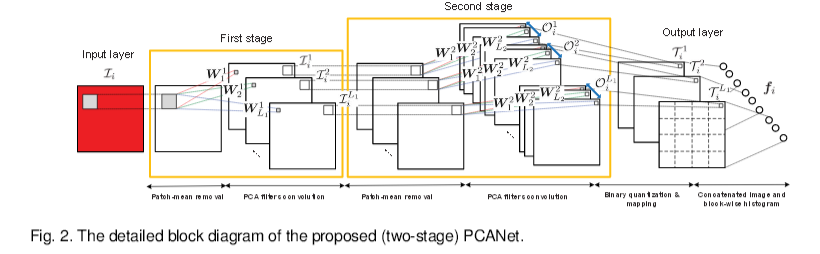
\includegraphics[scale=1.7,width=15cm]{pcanetstructure.png}
\vspace{-20pt}\caption{The Architecture of PCANet}\label{Figure: bspline}
\end{figure}




%\section{Experimental design}
\section{Datasets}
We will evaluate our new deep network in various tasks, and compare the results with the PCANet proposed in \cite{chan2015pcanet}. The potential tasks include:
\begin{itemize}
	\item Objection recognition on CIFAR10 dataset
	\item Digit recognition on MNIST dataset
	\item Face Verification on LFW dataset
\end{itemize}

%\subsection{Qualitative evaluation}

%\begin{table}\label{t1}
%\caption {Word aspect table}
%\centering
%\begin{tabular}{|l|l|l|l|}\hline
%Aspect1 & Aspect2 & ... & Aspect7 \\\hline
%word1 & word1 & ... & word1\\\hline
%word2 & word2 & ... & word2\\\hline
%word3 & word3 & ... & word3\\\hline
%word4 & word4 & ... & word4\\\hline
%word5 & word5 & ... & word5\\\hline
%\end{tabular}
%\end{table}
%
%\subsection{Quantitative evaluation}
%Test various algorithms on TripAdvisor data set to obtain the KL divergence, which measures the quality of the identified aspects \cite{wang2011structural}. KL divergence:
%\begin{equation}\label{eq1}
% D(p||q)= \sum_{x} p(x)log\frac{p(x)}{q(x)}
%\end{equation}
%where $p(x)$ represents the ground truth word distribution, $q(x)$ representing the word distribution learned by an algorithm. The smaller the divergence is, the closer the word distribution extracted by a given algorithm to the ground-truth is.
%
%\section{Why is related to machine learning?}
%Supervised machine learning and topic modeling are two main methods to extract aspects in reviews. In this project, we intend to implement some supervised learning algorithms and some topic modeling algorithms to extract aspects. Based on these research, we would try to improve the performance of the topic model. Therefore our project is highly related to machine learning.
%
%\section{Why are you the right team for implementing this plan?}
%Yin is a third year Ph.D student from the department of statistics and his research interest lies in bayesian statistics and machine learning. Now he is working on the topic modeling and sentiment analysis which relies on strong math and statistical background. This work is highly related to his current research area and he is confident with the mathematical part of this work. Renqin Cai is the first year graduate student in Computer Science, who is interested in machine learning and data mining. He has some backgrounds on supervised learning, unsupervised learning and topic model, which are main algorithms will be used in this project. Therefore, we believe we are qualified to finish such a project. 

\bibliography{mybib}{}
\bibliographystyle{ieeetr}
\end{document}
